\section{Experiments}
\label{sec:experiments}
% =============================================================================

\subsection{Setup}

\paragraph{Environments.}
We evaluate across five environments spanning both mechanisms.
The committed-action group comprises Pac-Man (Jumanji), Real-Time Tetris, and Snake,
each evaluated at simulation budgets of 32, 64, 96, and 128 simulations per move.
The clock group comprises Speed Hex (11$\times$11) and Speed Go (9$\times$9),
with budgets of 2, 8, 32, 128 and 16, 32, 64, 96 respectively.

\paragraph{Baselines.}
For committed-action environments we compare against \emph{always-$K$}
policies for each $K \in \Kset$ and a \emph{random} policy that samples
$K$ uniformly at each meta-step. For clock environments we additionally
compare against \emph{greedy} (always use the maximum simulation
budget) and \emph{midpeak} (a bell-curve schedule that concentrates
compute in the midgame, following common game-engine practice
\cite{baier2016time, huang2010timemanagement}). We tune the midpeak
shape separately at each evaluation budget and report the best result.

\paragraph{Base planner.}
For committed-action environments we use an AlphaZero checkpoint trained without
action delay ($K{=}1$) as the frozen base.
Cross-evaluation across checkpoints trained at each $K$ shows this checkpoint
is best overall (Appendix~\ref{app:cross_eval}).

\paragraph{Evaluation protocol.}
All results are averaged over 100 independent episode seeds; we report mean $\pm$ standard error.

\subsection{Main results}

\begin{figure}[t]
  \centering
  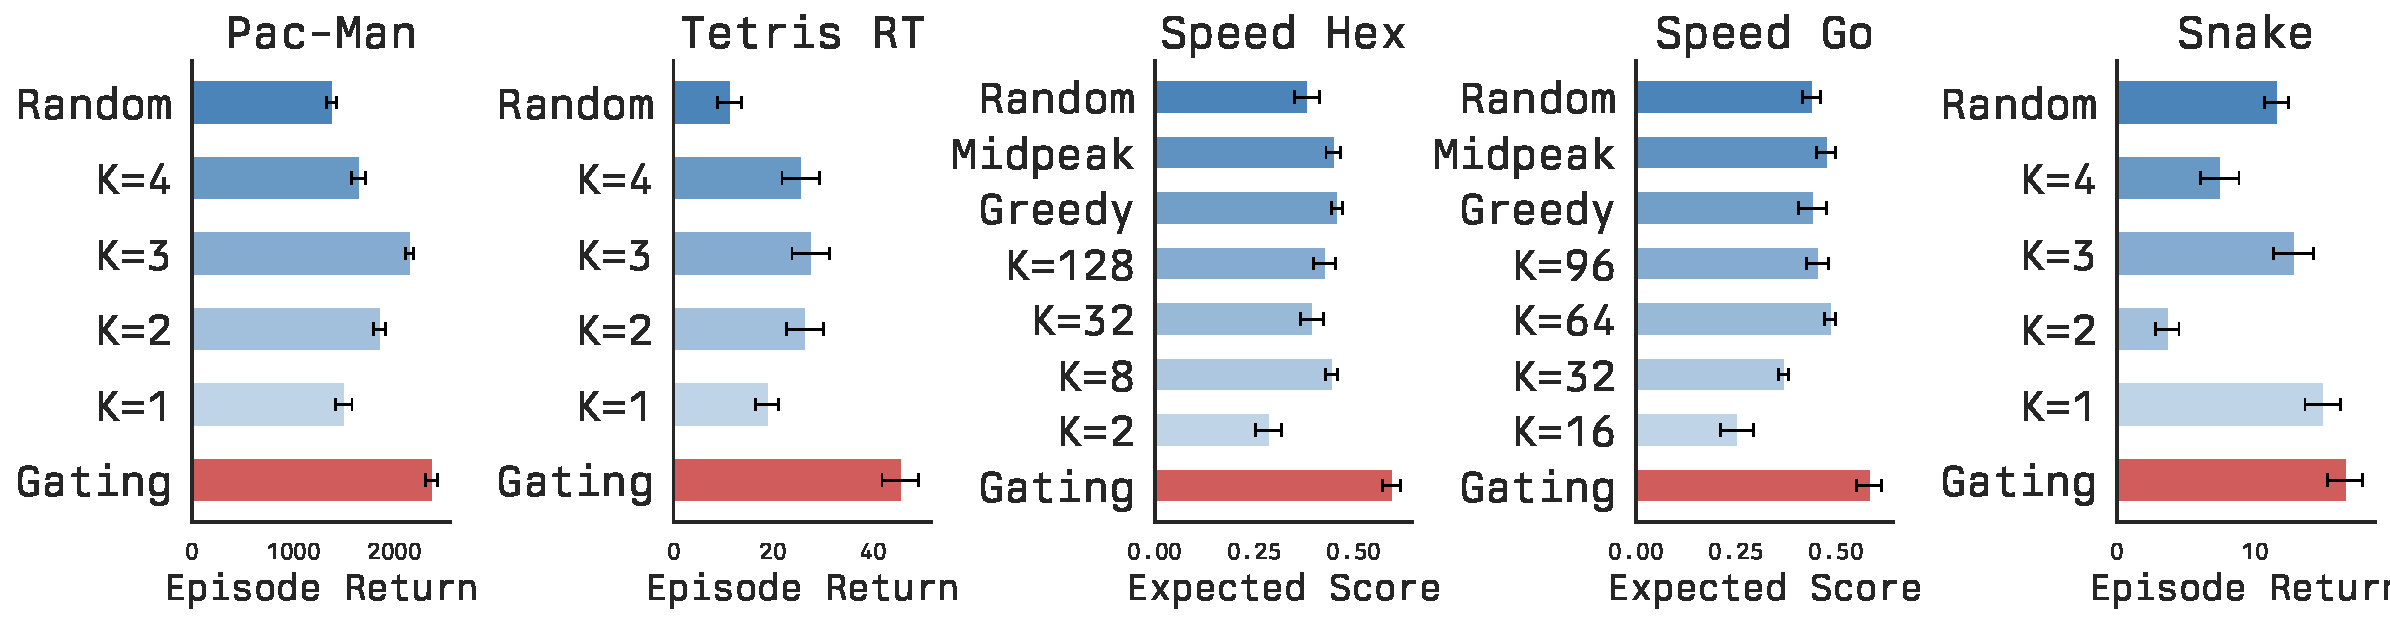
\includegraphics[width=\linewidth]{figures/main_results_horizontal.pdf}
  \caption{
    Across all five environments, the gating policy outperforms fixed-budget and
    heuristic baselines, showing that adaptive allocation matters more than
    committing to a single search budget. Bars show mean $\pm$\,SE over 100
    episodes; for Speed Hex and Speed Go, expected score is averaged over the
    shared sampled clock budgets.}
  \label{fig:main_results}
\end{figure}

The gating policy outperforms every fixed-budget baseline across all
five environments. In Pac-Man, the best fixed policy ($K{=}3$, 96
simulations per step) scores 2149, while the gate reaches 2370
($+10.3\%$) using about 49 simulations per frame on average. In
real-time Tetris, the best fixed policy ($K{=}3$) scores 27.6, while
the gate reaches 45.6 ($+65\%$). In Snake, the best fixed policy
($K{=}1$) scores 14.91, while the gate reaches 16.54 ($+10.9\%$) by
mostly reacting quickly and invoking deeper planning selectively.

For Speed Hex and Speed Go, we evaluate each policy at five sampled
clock budgets, $T \in \{300, 1200, 2300, 3500, 4800\}$, and average the
resulting head-to-head expected scores. Here $K{=}1,\dots,4$ denotes
the four simulation-budget options rather than committed-action lengths:
2/8/32/128 simulations for Speed Hex and 16/32/64/96 for Speed Go.
Against fixed-budget baselines and the greedy, midpeak, and random
heuristics, the gating policy remains above parity on average and
outperforms all of them overall.

Across environments, the learned gate does not collapse to a single
budget. It learns state- and budget-dependent allocation strategies
that beat both fixed policies and hand-designed heuristics
(Figure~\ref{fig:strategy}, Appendix Figure~\ref{fig:strategy_appendix}).
The random baseline falls well below every fixed-$K$ policy, confirming
that \emph{when} compute is allocated matters as much as how much.

\subsection{What triggers deeper planning?}

Across environments, the gate allocates more compute in higher-stakes
states, where a poor action is costly and extra search is more likely
to change the decision.

\paragraph{Pac-Man}

Ghost proximity correlates with lower chosen budgets in Pac-Man: the
policy prefers $K{=}1$ when the nearest ghost is far away, shifts
toward $K{=}2$ as the threat closes in, and reaches for $K{=}4$ at
extreme proximity. When ghosts are frightened, the policy reduces the
budget again.

\paragraph{Tetris}

Board density is the dominant feature in Tetris.
$K{=}1$ is selected almost exclusively on near-empty boards
(fill $\approx 0.05$, stack $\approx 3.5$ rows) where any reasonable placement is
acceptable.
$K{=}2$ and $K{=}4$ are selected on dense boards (fill
$\approx 0.25$--$0.32$, stacks $\approx 12$ rows) where placement
precision matters.
$K{=}3$ is never used ($0\%$), producing the bimodal ``react or plan deeply'' strategy
visible in Figure~\ref{fig:strategy}.
Piece type also modulates budget: the Z-piece ($\bar{K}{=}2.98{\scriptstyle\pm0.04}$)
and O- and T-pieces ($\bar{K}{=}2.88{\scriptstyle\pm0.04}$) receive the most
deliberation, while the J-piece ($\bar{K}{=}2.66{\scriptstyle\pm0.04}$) receives the
least, reflecting differences in placement geometry and expected outcome variance.

\paragraph{Snake}

Spatial constraint, rather than simple goal distance, is the main
trigger.
$K{=}1$ dominates on open boards, while $K{=}3$ appears when reachability drops,
local body density rises, and the snake has fewer safe continuations. $K{=}2$
occupies a milder regime associated with navigating toward more distant fruit on
otherwise open boards. Immediately after eating, when the body has just grown,
$K{=}3$ usage jumps from $3.2\%$ to $13.5\%$, indicating that the policy treats
body-growth events as a prospective spatial-risk signal.

\paragraph{Clock environments}

In the clocked PGX games, the relevant signal is the interaction
between board state and remaining time. Figure~\ref{fig:strategy} shows
that under the small clock budget ($T{=}300$), the policy heavily
favours the cheapest option, while under the larger budget
($T{=}4100$), it spreads mass more evenly across the four choices and
uses deeper search more often. Because the policy is trained across many
clock settings rather than tuned separately at each one, this shift is
evidence of budget-conditioned generalization. A strict-timeout Speed
Hex control in Appendix~\ref{app:hex_timeout_control} shows why we do
not use that variant as the main clock benchmark: once running out of
time becomes an immediate loss with no fallback, the task becomes much
easier and the main challenge is simply avoiding flag-falls.
Appendix~\ref{app:strategy_appendix} shows the full per-environment
strategy plots.

\begin{figure}[t]
  \centering
  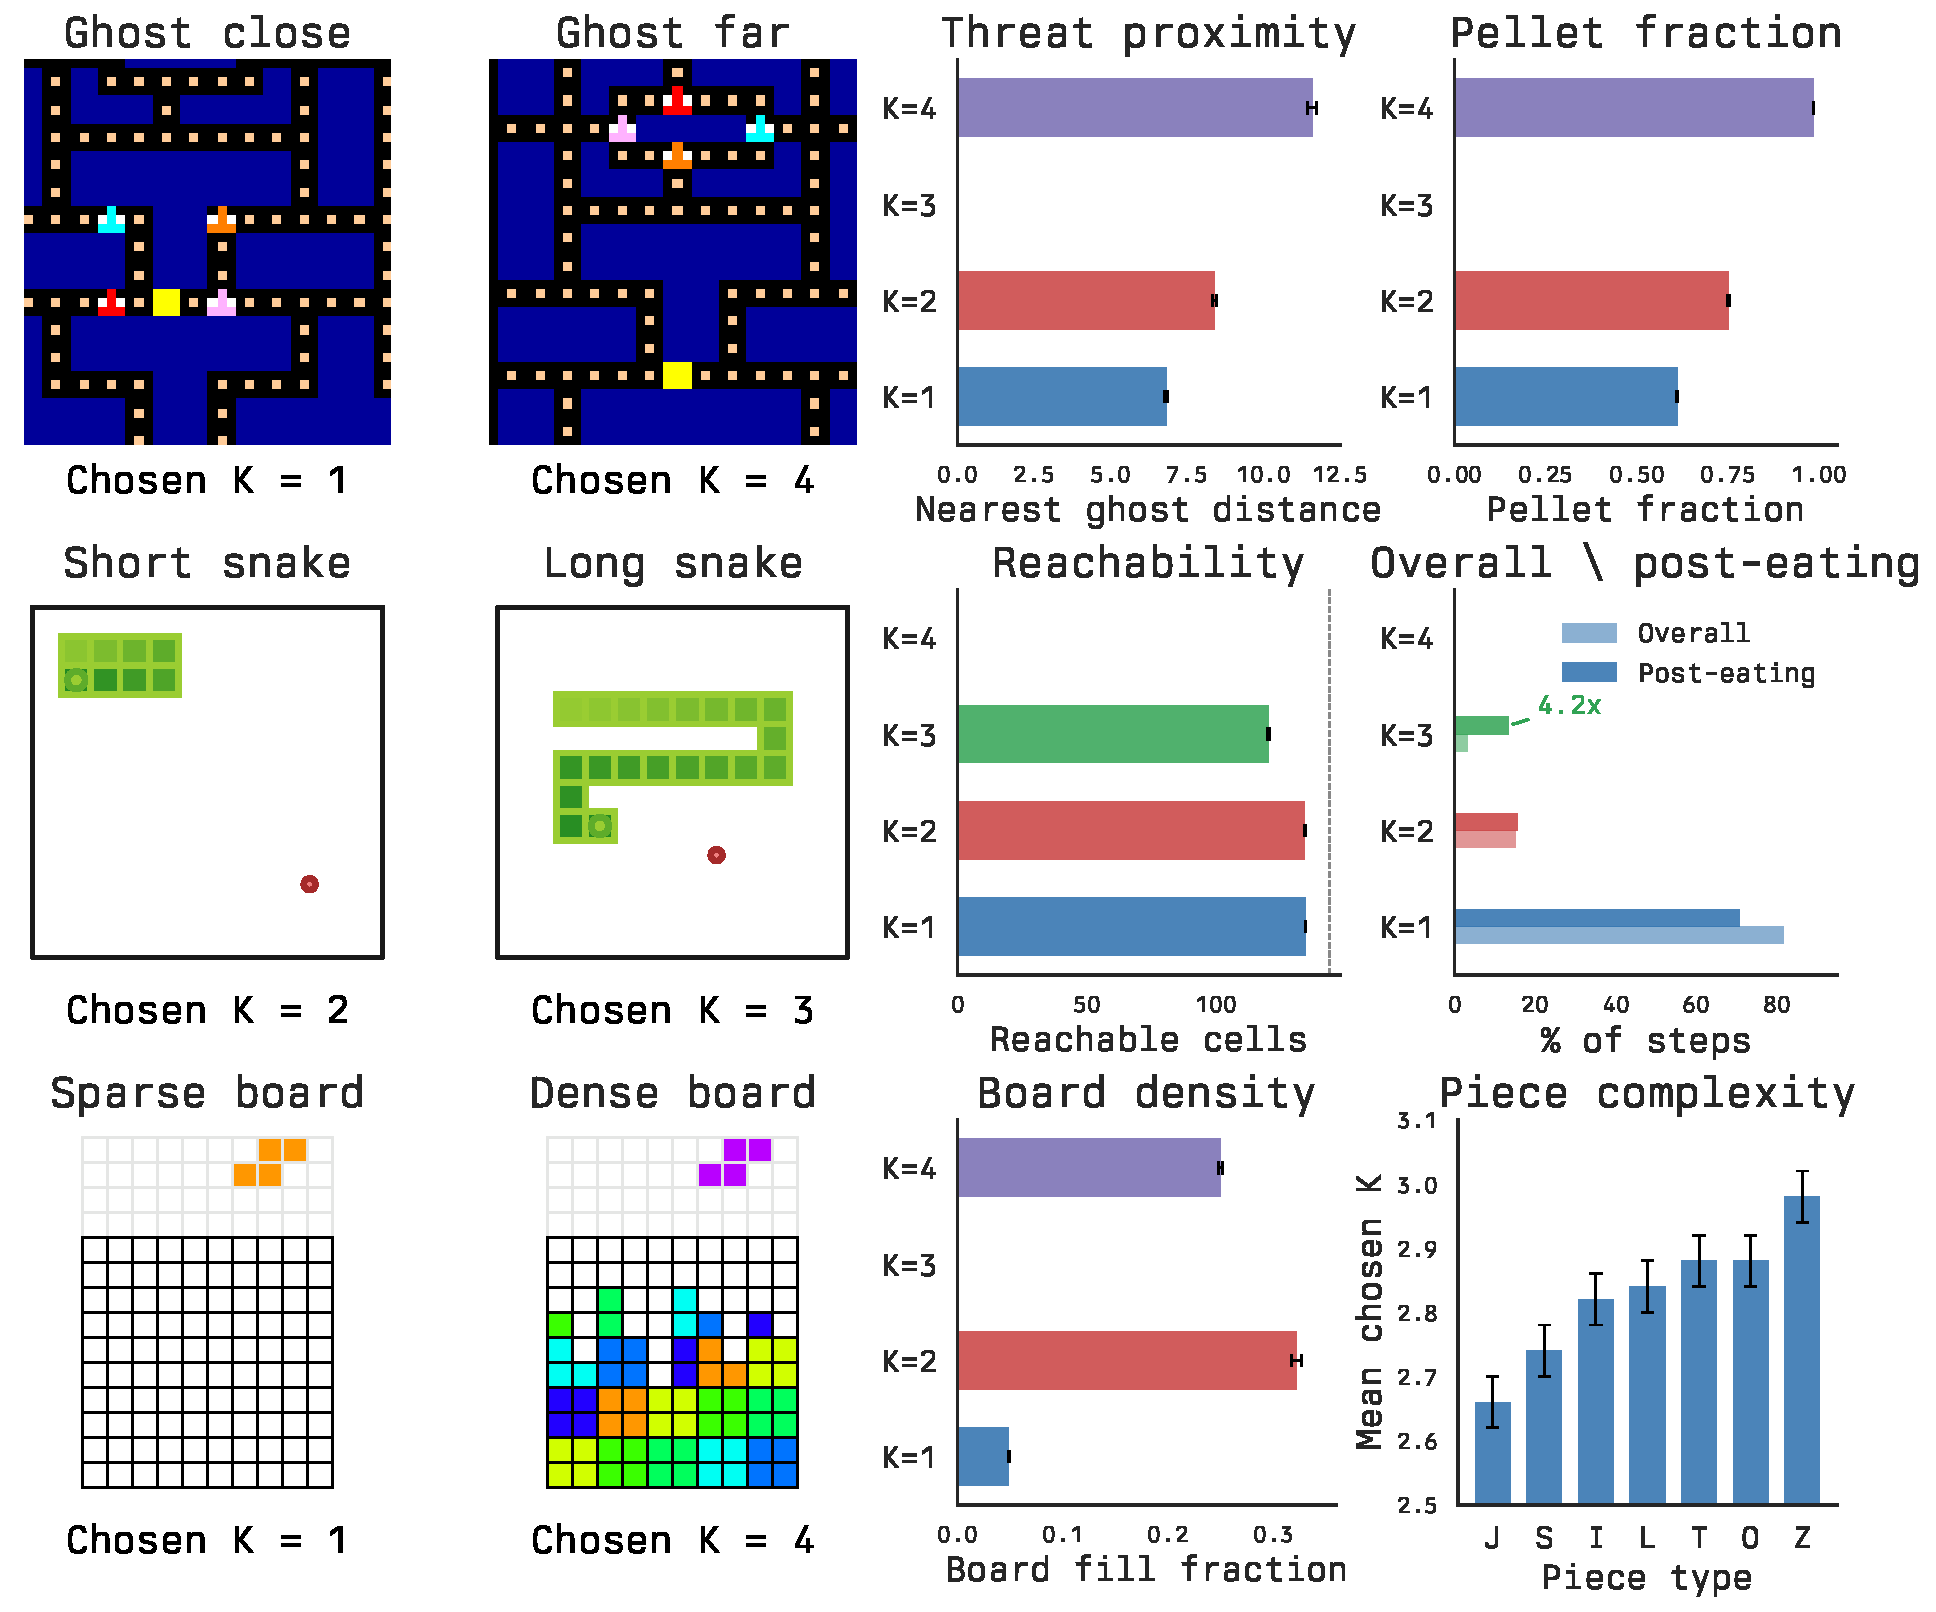
\includegraphics[width=\linewidth]{figures/interpretability_combined_alt.pdf}
  \caption{The policy plans deeply precisely when the state is dangerous or constrained.
    Across Pac-Man, Tetris, and Snake, larger chosen budgets are associated with
    higher threat, denser boards, or fewer safe continuations, indicating that
    the gate is responding to meaningful decision difficulty. Plots show state
    features conditioned on chosen budget $K$ (mean $\pm$\,1\,SE, 100 episodes).}
  \label{fig:interpretability}
\end{figure}



\begin{figure}[t]
  \centering
  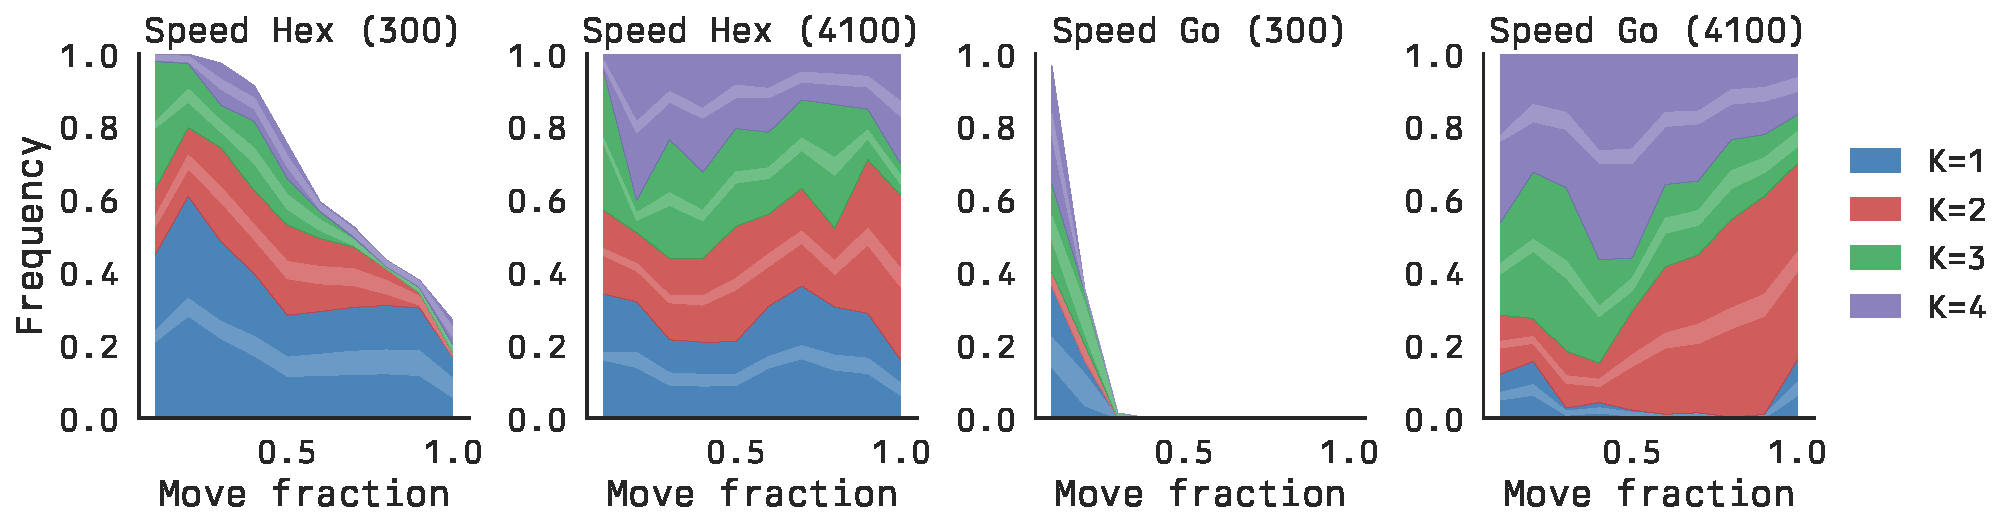
\includegraphics[width=1\linewidth]{figures/strategy_band.pdf}
  \caption{ In both Speed Hex and
    Speed Go, the learned policy is much more reactive under the small budget
    ($T{=}300$) and distributes mass toward deeper options once more clock is
    available ($T{=}4100$).}
  \label{fig:strategy}
\end{figure}


% =============================================================================
